\documentclass[conference]{IEEEtran}
\IEEEoverridecommandlockouts
% The preceding line is only needed to identify funding in the first footnote. If that is unneeded, please comment it out.
\usepackage{cite}
\usepackage{amsmath,amssymb,amsfonts}
\usepackage{algorithmic}
\usepackage{graphicx}
\usepackage{textcomp}
\usepackage{xcolor}
\usepackage{listings}

\definecolor{dkgreen}{rgb}{0,0.6,0}
\definecolor{gray}{rgb}{0.5,0.5,0.5}
\definecolor{mauve}{rgb}{0.58,0,0.82}

\lstset{frame=tb,
  language=java,
  aboveskip=3mm,
  belowskip=3mm,
  showstringspaces=false,
  columns=flexible,
  basicstyle={\small\ttfamily},
  numbers=none,
  numberstyle=\tiny\color{gray},
  keywordstyle=\color{blue},
  commentstyle=\color{dkgreen},
  stringstyle=\color{mauve},
  breaklines=true,
  breakatwhitespace=true,
  tabsize=3
}
\lstdefinestyle{mystyle}{
  numberstyle=\tiny\color{codegray},
  basicstyle=\footnotesize,
  breakatwhitespace=false,         
  breaklines=true,                 
  keepspaces=true,                 
  numbers=none,                    
  showspaces=false,                
  showstringspaces=false,
  showtabs=false,                  
  tabsize=2
}


\lstset{style= mystyle}

\def\BibTeX{{\rm B\kern-.05em{\sc i\kern-.025em b}\kern-.08em
    T\kern-.1667em\lower.7ex\hbox{E}\kern-.125emX}}
\begin{document}

\title{2D Polygon Triangulation}

\author{\IEEEauthorblockN{Ignacio Barquero Garcia$^{1}$, Jose Pablo Feng$^{2}$, Paul Villafuerte Beita$^{3}$}
\IEEEauthorblockA{\textit{Instituto Tecnologico de Costa Rica (ITCR)} \\
\textit
Cartago, Costa Rica \\
ibarqueroga@gmail.com, joseph.feng1@gmail.com,paulvillabeita@gmail.com}
}

\maketitle
\section{Abstract}
Abstract here
\section{Introduction}
Game figures and models that are visible in a computer screen and pretty much any other polygon can be deconstructed into triangles. This process is called \textbf{triangulation}. It consists of decomposing any polygon into triangles. In the following project, the chosen triangulation approach is the Ear Clipping path in order to "deconstruct" simple polygons into simpler polygons which are: triangles. In the following project, only 2D polygons will be tested and \textbf{non-simple polygons} (meaning one or more vertex are shared among various triangles or edges between two vertices that are intersected by other edge) are not triangulated in this project. Additionally, no vertices will be inserted.
$$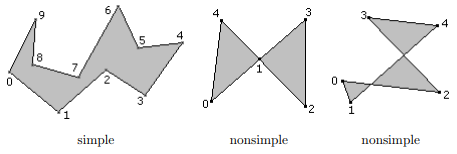
\includegraphics[scale=0.8]{nonsimpleExample}$$
\section{Polygon Triangulation}
Polygon Triangulation is the decomposition of a polygon in a surface or plane, into a set of triangles, with the restriction that each triangle side is entirely shared by two adjacent triangles. Triangulation can be applied to both convex and concave polygons. Concave polygons are those that have internal angles greater than 180 degrees, convex polygons are the opposite, internal angles sum 180 or less degrees. The Triangulation Theorem states that:
\begin{itemize}
    \item{Every simple polygon admits a triangulation}
\item{Every triangulation of an n-gon has exactly $n-2$ triangles}
\end{itemize}
$$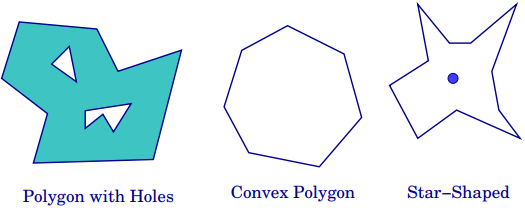
\includegraphics[scale=0.6]{Typeofpolygons}$$
\subsection{Triangulation Approaches}
    \subsubsection{\textbf{Non-Delaunay Algorithms}}
    \begin{itemize}
        \item{Greedy Triangulation}
        \item{Triangulation of Garey et.al}
        \item Ear Clipping / Ear Trimming
        \item{Radial Sweep}
    \end{itemize}
    \subsubsection{\textbf{Delaunay Algorithms}}
    \begin{itemize}
        \item Delaunay triangulation is proposed by B. Delaunay in 1934. Delaunay triangulation maximizes the minimum angles in triangles and avoids skinny triangles.
        \item Delaunay triangulation T of P is a triangulation of P such that the circum-circle of any traingle belonging to T does not contain points of P in its interior.
        \subsubsection{Properties}
        \begin{itemize}
            \item Local empty-circle property
            \item Max-min angle property
            \item Uniqueness
            \item Boundary property
        \end{itemize}
        \subsubsection{Algorithms}
        \begin{itemize}
            \item Incremental Algorithms
            \item Filliping Algorithm
            \item Plane Sweep Algorithm
            \item Divide and Conquer Algorithm
        \end{itemize}
    \end{itemize}
\section{Ear Clipping}
An ear of a polygon is a triangle formed by three consecutive vertices $V_{i0},V_{i1},$ and $V_{i2}$ for which $V_{i1}$ is a convex vertex. The line segment from $V_{i0}$ to $V_{i2}$ lies completely inside the polygon, and no vertices of the polygon are inside the triangle other than its components. The line segment between $V_{i0}$ and $V_{i2}$ is a diagonal of the polygon. The vertex $V_{i1}$ is called the ear tip. A triangle has only one ear and can be any of the triangle's vertices.
\section{Experimentation}
\subsection{Random points}
For the experimentation process, an input of the quantity of vertices is set and are going to be generated procedurally throughout the canvas.
\section{Code Analysis}
\begin{lstlisting}
    public void triangulatePolygon() {
      
        long start = System.currentTimeMillis(); //1
        boolean clockwise = isClockwise(points); //n
        int index = 0; //1
        if (points.size() < 3) { //1
            points.clear(); //1
        }else{
            while (points.size() > 2) { //n+1

              Point p1 = points.get((index + 0) % points.size());//1
              Point p2 = points.get((index + 1) % points.size());//1
              Point p3 = points.get((index + 2) % points.size());//1

            Vector v1 = new Vector(p2.x - p1.x, p2.y - p1.y);//1+1
            Vector v2 = new Vector(p3.x - p1.x, p3.y - p1.y);//1+1
                double cross = v1.cross(v2);//1+1
                Polygon triangle = new Polygon();
                triangle.addPoint(p1.x, p1.y); //1
                triangle.addPoint(p2.x, p2.y); //1
                triangle.addPoint(p3.x, p3.y); //1

                if (!clockwise && cross >= 0 && validTriangle(triangle, p1, p2, p3, points)) { //1+n
                    points.remove(p2);//1
                    triangles.add(triangle);//1
                }
                else if (clockwise && cross <= 0 && validTriangle(triangle, p1, p2, p3, points)) { //1+n
                    points.remove(p2);//1
                    triangles.add(triangle);//1
                }
                else {
                    index++;//1
                }
            }
            long end = System.currentTimeMillis();//1
            long time = end-start;//1+1
            long minutes = (time / 1000)  / 60;//1+1
            long seconds = (time / 1000) % 60;//1+1
            long milli = time - (seconds * 1000) - (minutes * 60000);//1
            String report = "Time taken: " + minutes + " min " + seconds + " sec " + milli +" ms" ; //1
            JOptionPane.showMessageDialog(null,report);
        }
    }
\end{lstlisting}

\begin{thebibliography}{}
\bibitem{Polygon Triangulation}Triangulation. (n.d.). Retrieved October 26, 2018, from http://mathworld.wolfram.com/Triangulation.html
\bibitem{Polygon Triangulation2} Subhash, S. (n.d.). Polygon Triangulation [Blog post]. Retrieved October 28, 2018, from https://www.cs.ucsb.edu/~suri/cs235/Triangulation.pdf
\bibitem{Concave Polygon}Concave Polygon Definition. (2011). Retrieved October 26, 2018, from https://www.mathopenref.com/polygonconcave.html
\bibitem{Triangulation Approaches}Varshosaz, M., Helali, H., \& Shojaee, D. (2017, April 7). The Methods of Triangulation - Geospatial World. Retrieved October 26, 2018, from https://www.geospatialworld.net/article/the-methods-of-triangulation/
\bibitem{Triangulation by Ear Clipping}Eberly, D. (2015, August 16). Triangulation By Ear Clipping [Blog post]. Retrieved October 28, 2018, from https://www.geometrictools.com/Documentation/TriangulationByEarClipping.pdf
\end{thebibliography}
\end{document}
